\documentclass{ximera}

\input{../preamble.tex}

\author{Gregory Hartman \and Matthew Carr}
\license{Creative Commons 3.0 By-NC}
\acknowledgement{https://github.com/APEXCalculus}

\begin{document}
\begin{exercise}

\outcome{Calculate limits using the limit laws.}
\outcome{Calculate limits of piecewise functions.}

\tag{limit} 
\tag{piecewise} 
\tag{continuous}

 Find 
  \[
  \lim_{x\to 3} f(x)
  \begin{prompt}
  = \answer{7}.
  \end{prompt}
  \]
  where
  \[
  f(x) = \begin{cases}x^2-x+1 & x\leq 3, \\
    2x+1 & x>3.
  \end{cases}
  \]
    \begin{hint}
     Both pieces of $f(x)$, $x^2-x+1$, for $x\leq3$, and $2x+1$, for $x>3$, are continuous for all $x$. However, for the limit $\lim_{x\to3}f(x)$ to exist, both the left-hand and the right-hand limits of $f(x)$ at $3$ must exist and be equal.
    \end{hint}
     \begin{hint}
    	Take a look at the graph of the function
    \begin{center}
     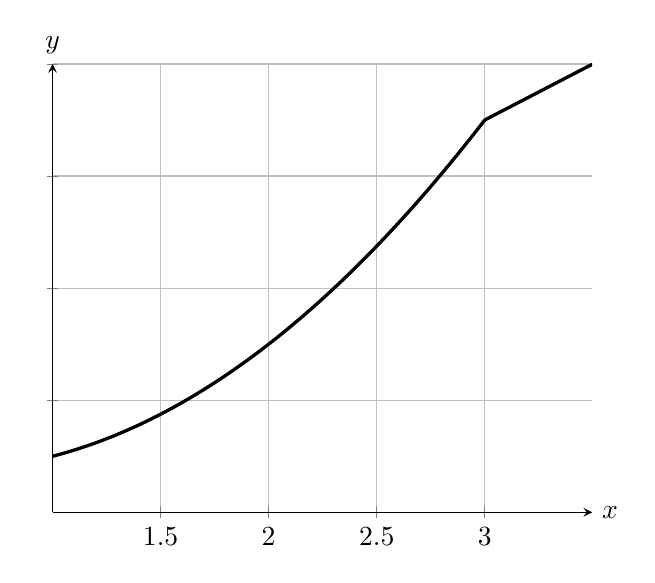
\begin{tikzpicture}
	\begin{axis}
	[ymin=0,ymax=8, axis lines=center,xlabel=$x$,ylabel=$y$,every axis y 
	label/.style={at=(current axis.above origin),anchor=south},every axis x label/.style={at=(current axis.right of origin),anchor=west},
	domain=-1:4,
	yticklabels={},
	ymajorgrids=true,
	grid = major
	]
	\addplot[domain=1:5,very thick,smooth,samples=600]
	{(!(\x>3))*(\x^2-\x+1)+(\x>3)*(2*\x+1)};
	\end{axis}
       \end{tikzpicture}      
      \end{center} 
    \end{hint}
    \begin{hint}
     Evaluating $\lim_{x\to3^{+}}f(x)$ we see that it is equal to $7$. This follows because, for $x>3$, we are on the piece of $f(x)$ given by $2x+1$ and the limit $\lim_{x\to3}\left({2x+1}\right)=2\cdot\lim_{x\to 3}(x)+\lim_{x\to3}\left({1}\right)=7$, certainly. On the other hand, evaluating $\lim_{x\to3^{-}}f(x)$ we see it is equal to $7$. This follows because, for $x\leq3$, we are on the piece of $f(x)$ given by $x^2-x+1$ and the limit $\lim_{x\to3}\left({x^2-x+1}\right)=\left({\lim_{x\to3}(x)}\right)^2-\lim_{x\to 3}(x)+\lim_{x\to3}\left({1}\right)=7$, certainly. These are equal, so the limit exists is equal to $7$.
    \end{hint}
\end{exercise}

\end{document}
